\section{Passerelle intelligente}

\begin{frame}{Architecture réseau}
  \begin{figure}
    \centering
    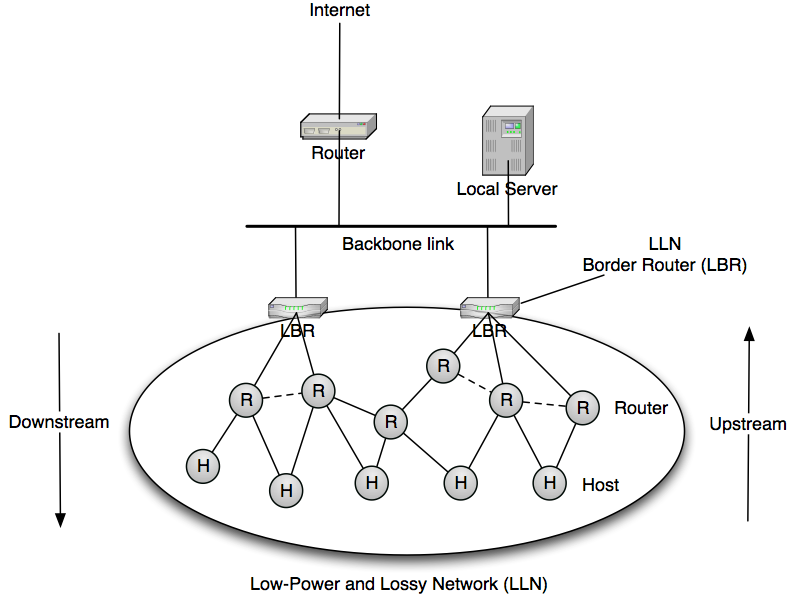
\includegraphics[scale=.3]{figures/rpl.png}
  \end{figure}
  \pnote{
    Il est à noter que les routeurs peuvent aussi héberger des serveurs applicatifs
  }
\end{frame}

\begin{frame}{Protocoles pour les LLNs}
  \begin{figure}
    \centering
    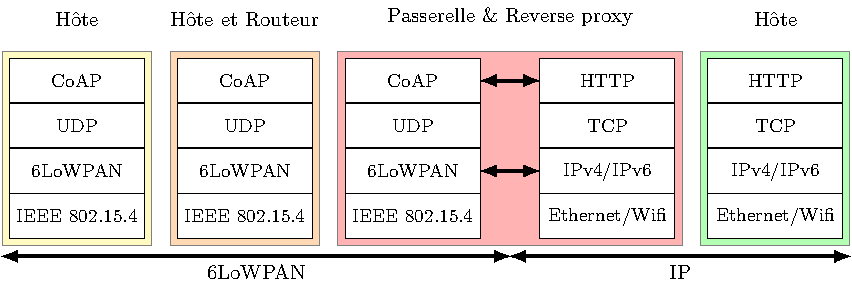
\includegraphics[width=\textwidth]{figures/network_stack_slides.pdf}
  \end{figure}

  \pnote{
    - Propos général : les protocoles classiques sont adaptés aux réseaux de capteurs pour en faire des membres à part entières de l'Internet.
  }

  \pnote{
    - IEEE 802.15.4: Couche Physique et MAC; topo maillé/étoilée; Faible cout
  }
  \pnote{
    - 6LoWPAN: Compression IPv6
  }
  \pnote{
    - RPL: Produit les routes montantes et descendantes;
  }
  \pnote{
    - CoAP: Couche applicative; REST; UDP
  }
\end{frame}

\begin{frame}{Rôle de la passerelle}
  \begin{block}{Couche physique et liaison: \ieee{}}
    \begin{itemize}
      \item PAN coordinator
    \end{itemize}
  \end{block}
  \begin{block}{Couche réseau: 6LoWPAN}
    \begin{itemize}
      \item Compression IPv6
    \end{itemize}
  \end{block}
  \begin{alertblock}{Protocole de routage: RPL}
    \begin{itemize}
      \item Racine du DODAG (MP2P/P2MP)
      \item Routeur de bordure (LBR)
    \end{itemize}
  \end{alertblock}
  \begin{alertblock}{Protocole applicatif: CoAP}
    \begin{itemize}
      \item Traduction de protocole (HTTP/CoAP)
      \item Proxy inverse
    \end{itemize}
  \end{alertblock}
\end{frame}

\begin{frame}{Problématiques}

  \begin{block}{Prévision de l'impact du trafic}
    \begin{itemize}
      \item Provisionnement du réseau
      \item Surveillance matérielle et fonctionnelle continue
      \item Anticipation des pannes
    \end{itemize}
  \end{block}

  \begin{block}{Optimisation de l'utilisation des ressources}
    \begin{itemize}
      \item Économie de bande-passante et d'énergie
      \item Améliorer la rapidité du traitement
    \end{itemize}
  \end{block}

  \pnote{
    - Avoir une idée de trafic permet de dimensionner son réseau correctement (couverture, routeur intermédiaire)
    Ce qui apporte des gains de fiabilité et aide aux diagnostiques de problèmes.
  }
  \pnote{
    - Suivi de la disponibilité matérielle (un noeud mort) ou fonctionnelle (tout un étage est mort)
  }
  \pnote{
    - Prévoir l'évolution de métriques pour faire des interventions: Niveau de batterie, carte sd saturée
  }
  \pnote{---}
  \pnote{
    - Accorder les demandes des utilisateurs. Les rythmes de requetes importantes.
  }
  \pnote{
    - Servir une réponse depuis la passerelle va plus vite que depuis les noeuds
  }
\end{frame}

% % Annonce des contributions

\begin{frame}\frametitle{Contributions}

  \begin{alertblock}{Supervision passive}
    \begin{itemize}
      \item Observe le trafic au niveau du routeur de bordure
      \item Fournit une estimation de l'utilisation de la radio permettant de déduire une partie de la consommation énergétique
    \end{itemize}
  \end{alertblock}

  \begin{alertblock}{Reverse proxy adaptatif}
    \begin{itemize}
      \item Régule les temps de validité des réponses en cache au niveau de la passerelle
      \item Offre un compromis entre satisfaction des utilisateurs et économies d'énergie
    \end{itemize}
  \end{alertblock}

  \pnote{
    Comment ajouter des services dans le dernier noeud non contraints qui est à la bordure du réseau standard ?
  }
  \pnote{
    - Dire que l'on a d'autres contributions mais que cette présentation se concentre sur celles présentées pour la passerelle.
  }

\end{frame}
